\documentclass[border=12pt]{standalone}
  \usepackage{tikz}
  \usepackage{xcolor}
  \usepackage[T1]{fontenc}

  \usetikzlibrary{
    shapes.symbols,
    positioning,
    calc
  }

\definecolor{hardware}{RGB}{64,64,64}
\definecolor{hvcolor}{RGB}{185,185,185}
\definecolor{appcolor}{RGB}{67,114,196}   % blue
\definecolor{oscolor}{RGB}{82,153,53}     % green
\definecolor{kernelcolor}{RGB}{192,39,39} % red

\tikzset{
  pics/vm/.style args={#1}{
    code={
      \path[draw,fill=appcolor]
        (0,0) coordinate (topleft_app_#1)
          -- ++(2,0)  coordinate (topright_app_#1)
          -- ++(0,-1) coordinate (bottomright_app_#1)
          -- ++(-2,0) coordinate (bottomleft_app_#1)
          -- cycle
      ;
      \path[]
        ($(topleft_app_#1)!0.5!(bottomright_app_#1)$) node[] (label_app_#1) {Apps #1}
      ;
      \path[draw,fill=oscolor]
        ($(topleft_app_#1)+(0,-1.05)$) coordinate (topleft_os_#1)
          -- ++(2,0) coordinate (topright_os_#1) 
          -- ++(0,-1) coordinate (bottomright_os_#1)
          -- ++(-2,0) coordinate (bottomleft_os_#1)
          -- cycle
      ;
      \path[]
        ($(topleft_os_#1)!0.5!(bottomright_os_#1)$) node[label={[align=center]center:OS #1\\{\ttfamily\small (\textbackslash bin:\textbackslash lib)}}] (label_os_#1) {}
      ;
      \path[draw,fill=kernelcolor]
        ($(topleft_os_#1)+(0,-1.05)$) coordinate (topleft_kernel_#1)
          -- ++(2,0) coordinate (topright_kernel_#1) 
          -- ++(0,-1) coordinate (bottomright_kernel_#1)
          -- ++(-2,0) coordinate (bottomleft_kernel_#1)
          -- cycle
      ;
      \path[]
        ($(topleft_kernel_#1)!0.5!(bottomright_kernel_#1)$) node[] (label_kernel_#1) {OS #1 kernel}
      ;
    }
  }
}

\tikzset{
  pics/container/.style args={#1}{
    code={
      \path[draw,fill=appcolor]
        (0,0) coordinate (container_topleft_app_#1)
          -- ++(2,0) coordinate (container_topright_app_#1) 
          -- ++(0,-1) coordinate (container_bottomright_app_#1)
          -- ++(-2,0) coordinate (container_bottomleft_app_#1)
          -- cycle
      ;
      \path[]
        ($(container_topleft_app_#1)!0.5!(container_bottomright_app_#1)$) node[] (container_label_app_#1) {Apps #1}
      ;
      \path[draw,fill=oscolor]
        ($(container_topleft_app_#1)+(0,-1.05)$) coordinate (container_topleft_os_#1)
          -- ++(2,0) coordinate (container_topright_os_#1)
          -- ++(0,-1) coordinate (container_bottomright_os_#1)
          -- ++(-2,0) coordinate (container_bottomleft_os_#1)
          -- cycle
      ;
      \path[]
        ($(container_topleft_os_#1)!0.5!(container_bottomright_os_#1)$) node[label={[align=center]center:OS #1\\{\ttfamily\small (\textbackslash bin:\textbackslash lib)}}] (label_os_#1) {}
      ;
    }
  }
}

\begin{document}
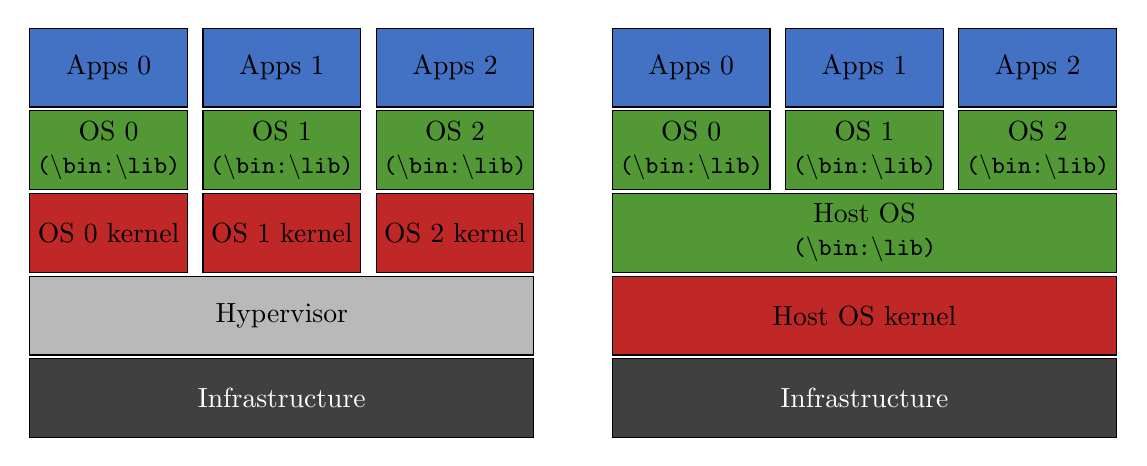
\begin{tikzpicture}[x=1cm, y=1cm]

\path[draw] (0,0) pic {vm={0}};
\path[draw] ($(topleft_app_0)+(2.2,0)$) pic {vm={1}};
\path[draw] ($(topleft_app_1)+(2.2,0)$) pic {vm={2}};

\path[draw,fill=hvcolor]
  let
    \p{hypervisor_topleft} = ($(bottomleft_kernel_0)+(0,-0.05)$),
    \p{hypervisor_bottomright} = ($(bottomright_kernel_2)+(0,-1.05)$),
  in
  (\x{hypervisor_topleft}, \y{hypervisor_topleft}) coordinate (hv_topleft) --
    (\x{hypervisor_bottomright},\y{hypervisor_topleft}) coordinate (hv_topright) --
    (\x{hypervisor_bottomright},\y{hypervisor_bottomright}) coordinate (hv_bottomright) --
    (\x{hypervisor_topleft},\y{hypervisor_bottomright}) coordinate (hv_bottomleft) --
    cycle
;
\path[]
  ($(hv_topleft)!0.5!(hv_bottomright)$) node[] (hv) {Hypervisor}
;

\path[draw,fill=hardware]
  let
    \p{hardware_topleft} = ($(hv_bottomleft)+(0,-0.05)$),
    \p{hardware_bottomright} = ($(hv_bottomright)+(0,-1.05)$),
  in
  (\x{hardware_topleft}, \y{hardware_topleft}) coordinate (hw_topleft) --
    (\x{hardware_bottomright},\y{hardware_topleft}) --
    (\x{hardware_bottomright},\y{hardware_bottomright}) coordinate (hw_bottomright) --
    (\x{hardware_topleft},\y{hardware_bottomright}) --
    cycle
;
\path[draw,text=white]
  ($(hw_topleft)!0.5!(hw_bottomright)$) node[] (machine) {Infrastructure}
;

\path[draw] ($(topright_app_2)+(1,0)$) pic {container={0}};
\path[draw] ($(container_topleft_app_0)+(2.2,0)$) pic {container={1}};
\path[draw] ($(container_topleft_app_1)+(2.2,0)$) pic {container={2}};

\path[draw,fill=oscolor]
  let
    \p{container_system_os_topleft} = ($(container_bottomleft_os_0)+(0,-0.05)$),
    \p{container_system_os_bottomright} = ($(container_bottomright_os_2)+(0,-1.05)$),
  in
  (\x{container_system_os_topleft}, \y{container_system_os_topleft}) coordinate (cso_topleft) --
    (\x{container_system_os_bottomright},\y{container_system_os_topleft}) coordinate (cso_topright) --
    (\x{container_system_os_bottomright},\y{container_system_os_bottomright}) coordinate (cso_bottomright) --
    (\x{container_system_os_topleft},\y{container_system_os_bottomright}) coordinate (cso_bottomleft) --
    cycle
;
\path[]
  ($(cso_topleft)!0.5!(cso_bottomright)$) node[label={[align=center]center:Host OS\\{\ttfamily\small (\textbackslash bin:\textbackslash lib)}}] (cso) {}
;

\path[draw,fill=kernelcolor]
  let
    \p{host_kernel_topleft} = ($(cso_bottomleft)+(0,-0.05)$),
    \p{host_kernel_bottomright} = ($(cso_bottomright)+(0,-1.05)$),
  in
  (\x{host_kernel_topleft}, \y{host_kernel_topleft}) coordinate (hk_topleft) --
    (\x{host_kernel_bottomright},\y{host_kernel_topleft}) coordinate (hk_topright) --
    (\x{host_kernel_bottomright},\y{host_kernel_bottomright}) coordinate (hk_bottomright) --
    (\x{host_kernel_topleft},\y{host_kernel_bottomright}) coordinate (hk_bottomleft) --
    cycle
;
\path[]
  ($(hk_topleft)!0.5!(hk_bottomright)$) node[] (hk) {Host OS kernel}
;

\path[draw,fill=hardware]
  let
    \p{container_hardware_topleft} = ($(hk_bottomleft)+(0,-0.05)$),
    \p{container_hardware_bottomright} = ($(hk_bottomright)+(0,-1.05)$),
  in
  (\x{container_hardware_topleft}, \y{container_hardware_topleft}) coordinate (container_hw_topleft) --
    (\x{container_hardware_bottomright},\y{container_hardware_topleft}) --
    (\x{container_hardware_bottomright},\y{container_hardware_bottomright}) coordinate (container_hw_bottomright) --
    (\x{container_hardware_topleft},\y{container_hardware_bottomright}) --
    cycle
;
\path[draw,text=white]
  ($(container_hw_topleft)!0.5!(container_hw_bottomright)$) node[] (container_machine) {Infrastructure}
;

\end{tikzpicture}
\end{document}

